\section{Detection}\label{sec:dessensor}
In \cref{bestchoice} the ultra sonic sensors were strongly discouraged due to interference. This leaves the infrared distance sensors as the remaining option, in light of this, the design will only consider infrared motion detection. \\

As written in \cref{cone} the sensors have faulty measurements in certain areas of their fields of view. The sensors' faulty measurements can be used to determine in which of three different areas of the field of view the target was detected in. \\

The areas, shown in \cref{sensorsections2}, are determined by the distance reading. First, any reading above 700 millimeters is considered noise, and is disregarded. If a reading occurs between 700 millimeters and 300 millimeters, the target is in one of the outer areas, denoted on \cref{sensorsections2} as O. If a reading is below 300 millimeters, it is in the inner zone, denoted by I. This, however, limits the turret to be placed at a specific distance from the tracks as the readings change with the distance.

\begin{figure}[H]
\begin{center}
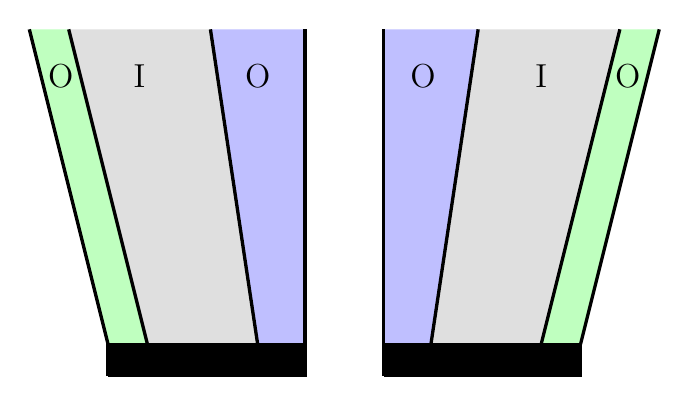
\begin{tikzpicture}

\fill[fill=green!25] (0,0.4) -- (-1,4.4) -- (-0.5,4.4) -- (0.5,0.4) -- (0,0.4); 
\fill[fill=gray!25] (0.5,0.4) -- (-0.5,4.4) -- (1.3,4.4) -- (1.9,0.4) -- (0.5,0.4);
\fill[fill=blue!25] (1.9,0.4) -- (1.3,4.4) -- (2.5,4.4) -- (2.5,0.4) -- (2,0.4);
\fill[fill=black] (0,0) -- (0,0.4) -- (2.5,0.4) -- (2.5,0) -- (0,0);

\fill[fill=green!25] (6,0.4) -- (7,4.4) -- (6.5,4.4) -- (5.5,0.4) -- (6,0.4);
\fill[fill=gray!25] (5.5,0.4) -- (6.5,4.4) -- (4.7,4.4) -- (4.1,0.4) -- (5.5,0.4);
\fill[fill=blue!25] (4.1,0.4) -- (4.7,4.4) -- (3.5,4.4) -- (3.5,0.4) -- (4.1,0.4);
\fill[fill=black] (3.5,0) -- (3.5,0.4) -- (6,0.4) -- (6,0) -- (3.5,0);

\draw[very thick] (0,0) -- (0,0.4) -- (2.5,0.4) -- (2.5,0) -- (0,0);
\draw[very thick] (3.5,0) -- (3.5,0.4) -- (6,0.4) -- (6,0) -- (3.5,0);

\draw[very thick] (2.5,0.4) -- (2.5,4.4);
\draw[very thick] (1.9,0.4) -- (1.3,4.4);
\draw[very thick] (0.5,0.4) -- (-0.5,4.4);
\draw[very thick] (0.0,0.4) -- (-1,4.4);

\draw[very thick] (3.5,0.4) -- (3.5,4.4);
\draw[very thick] (4.1,0.4) -- (4.7,4.4);
\draw[very thick] (5.5,0.4) -- (6.5,4.4);
\draw[very thick] (6,0.4) -- (7,4.4);

\node at (-0.6,3.8) {\large O};
\node at (0.4,3.8) {\large I};
\node at (1.9,3.8) {\large O};



\node at (4,3.8) {\large O};
\node at (5.5,3.8) {\large I};
\node at (6.6,3.8) {\large O};


%\draw[very thick] (2,4.8) -- (4,4.8);
%\draw[very thick] (2,4.6) -- (2,5);
%\draw[very thick] (4,4.6) -- (4,5);
%\node at (3,5.1) {\normalsize TRAIN};


\end{tikzpicture}
\caption{Infrared sensor detection zones.}
\label{sensorsections2}
\end{center}
\end{figure}

As the motors rotation is specified in degrees, the zones should also be interpreted as an offset in degrees. Interpreting the zones into offsets is met by two challenges. The first challenge is to translate the zones into offsets. The offset of each area was found by measuring the distance from the rotation point of the turret to the train tracks and then measuring the offset of the train as it just shifted to a new area. Then the inverse tangent was used to calculate the offset, measured in degrees, of each area, which can be seen in \cref{areas}. The areas listed in the table can be seen in figure \cref{sensarea1}. The distance from the turret to the track was 470 millimeters, as this put the sensors in their optimal position.

\begin{table}[H]
\centering
\begin{tabular}{|l|l|l|l|l|l|}
\hline
\textbf{Area}   & -2     & -1    & 0    & 1    & 2     \\ \hline
\textbf{Degrees} & 17.37 & 7.52 & -1.058 & -9.78 & -20.74 \\ \hline
\end{tabular}
\caption{Sensor areas.}
\label{areas}
\end{table}

The second challenge is to determine which of the outer zones the target was spotted in. At the highest tested speed, the target travelled 63.3 degrees per second. Since the inner zone is 11.19 degrees, the target will pass through the zone in 177 milliseconds. Since the sensors are polled at speeds as low as 6 milliseconds, see \cref{pollingrate}, a target will not pass by the inner zone without being spotted. Therefore, any reading in an outer zone, which is not immediately preceded by its corresponding inner zone, is considered to be the outermost of the outer zones, unless the other sensor has already spotted the target. A reading in zone 0, the smallest zone, requires a polling time below 42 milliseconds. \\

This gives the combined field of view illustrated in \cref{sensarea1}. Since the outermost outer zones were small areas, they were considered an extension of the inner zone. The inner zones are labelled $-2$ and $2$, the innermost outer zones are labelled $-1$ and $1$, with negative numbers for left side and positive for right side. If the target is spotted in both zone $-1$ and $1$, it is instead read as being in zone $0$, which indicates that the train is in the middle of the combined field of view of the two sensors.

\begin{figure}[H]
\begin{center}
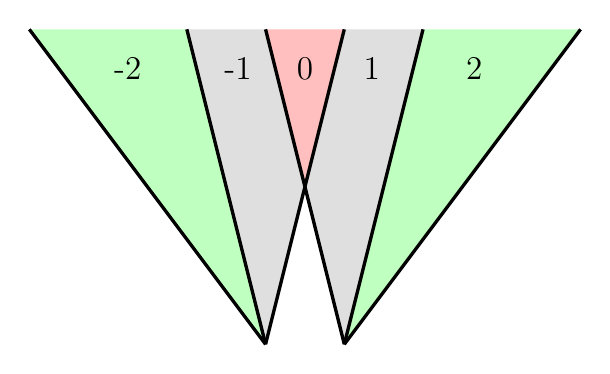
\begin{tikzpicture}
\fill[fill=gray!25] (8,0) -- (8.5,2) -- (8,4) -- (7,4) -- (8,0); % Left block (center)
\fill[fill=gray!25] (9,0) -- (8.5,2) -- (9,4) -- (10,4) -- (9,0); % Right block (center)
\fill[fill=red!25] (8.5,2) -- (8,4) -- (9,4) -- (8.5,2); % Center block
\fill[fill=green!25] (8,0) -- (5,4) -- (7,4) -- (8,0); % Left block
\fill[fill=green!25] (9,0) -- (12,4) -- (10,4) -- (9,0); % Right block
\draw[very thick] (9,0) -- (8,4);
\draw[very thick] (9,0) -- (10,4);
\draw[very thick] (9,0) -- (12,4);
\draw[very thick] (8,0) -- (9,4);
\draw[very thick] (8,0) -- (7,4);
\draw[very thick] (8,0) -- (5,4);
\node at (6.25,3.5) {\large-2};
\node at (7.65, 3.5) {\large-1};
\node at (8.5, 3.5) {\large0};
\node at (9.35, 3.5) {\large1};
\node at (10.65, 3.5) {\large2};
\end{tikzpicture}
\caption{Combined field of view.}
\label{sensarea1}
\end{center}
\end{figure}

\paragraph{Resting Policy} ~\\
In \cref{sec:requirements}, the second requirement concerns ways the turret can find a target in the observable area. As the setup consists of the two infrared sensors, observing the entire observable area at once is not possible. In the setup the target will always come from one direction and as such searching the entire area is not an optimal solution. Given the counterclockwise rotation, making the turret rest at the rightmost position is the best choice for a key point, as this ensures that the target is spotted at the time it enters the observable area.
